%\documentclass[handout]{beamer}
%\usepackage{pgfpages}
%\pgfpagesuselayout{4 on 1}[a4paper, landscape, border shrink=5mm]
%\pgfpageslogicalpageoptions{1}{border code=\pgfusepath{stroke}}
%\pgfpageslogicalpageoptions{2}{border code=\pgfusepath{stroke}}
%\pgfpageslogicalpageoptions{3}{border code=\pgfusepath{stroke}}
%\pgfpageslogicalpageoptions{4}{border code=\pgfusepath{stroke}}
\documentclass{beamer}
\usetheme{nesl}  % Now it's a beamer presentation with the NESL theme!
\usepackage{tikz}
\usetikzlibrary{shapes,arrows}
\usepackage{url}
\usepackage{movie15}
\usepackage{verbatim}

% Make a new command that will make a new subsection and a frame with the same title
\newcommand{\fst}[2]{\subsection{#1}\frame{\frametitle{#1} #2}}

% Standard LaTeX stuff - note the optional abbreviated title being provided
\title{Report on the development of \\GSI/WRF 4DVAR capability}
\author[Zhang]{Xin Zhang}

\date{~\\
~\\ACAPS Project Report\\
  ~\\
  ~\\
 \tiny{NCAR is sponsored by the National Science Foundation}
}

\institute[NCAR Earth System Laboratory]{
% \url{xinzhang@ucar.edu} \\
   NCAR Earth System Laboratory \\
%  \url{ook@ucw.cz}\\
%  Charles University, Prague
}

% We want the NSF department logo
\logo{
\includegraphics[height=.5in]{nsf1.jpg}}


\begin{document}

% The title page
\frame{\titlepage}

%%%%%%%%%%%%%%%%%%%%%%%%%
\section{Introduction}

\frame{
\frametitle{Current Status}
\begin{itemize}
	\item This presentation reports to the status of the development of GSI/WRF 4DVAR as implemented in Boulder's version of January 2011\pause
	\item The WRF tangent linear and adjoint codes (hereafter, WRFPLUS)  have been updated to be consistent with the latest WRF repository codes \pause
	\item The Major development in GSI had finished, GSI codes had been coupled with the latest WRFPLUS \pause
	\item Because the parallelization of the latest WRFPLUS is still on going, only 1 processor parallel run can be done at this moment
	\end{itemize}
}


%%%%%%%%%%%%%%%%%%%%%%%%%%%%%%%%%
\section{Upgrades of WRFPLUS}

\fst{Major Improvements}{
\begin{itemize}
   	\item New WRF adjoint and tangent linear codes based on the latest WRF repository codes. \pause
	\item Testing the code on various  platforms and compilers ( IBM, Linux, Mac : xlf, g95, pgi, intel). \pause
	\item Add capability to do tangent linear and adjoint test over any length of time window. \pause 
	\item Add option to control if all inputs and outputs were happen in disk or memory, so WRFPLUS can be used as a standalone tool or as a component in 4DVAR system.
\end{itemize}
}

\begin{frame}[fragile]
\frametitle{Sample Tangent Linear and Adjoint Check }
\setbeamercolor{postit}{fg=black, bg=yellow}
\begin{beamerboxesrounded}[ lower=postit,shadow=true]{Tangent linear check}
\begin{verbatim}
 ...
 tl_check: alpha=.1000E-04  coef=0.10000447262220E+01  
 tl_check: alpha=.1000E-05  coef=0.99999981575068E+00
 tl_check: alpha=.1000E-06  coef=0.99999998152933E+00
 tl_check: alpha=.1000E-07  coef=0.99999990980017E+00
 tl_check: alpha=.1000E-08  coef=0.99999956711797E+00
 ...
\end{verbatim}
\end{beamerboxesrounded}
\begin{beamerboxesrounded}[ lower=postit,shadow=true]{Adjoint check}
\begin{verbatim}
 ad_check: VAL_TL:    0.42476489986911E+11
 ad_check: VAL_AD:    0.42476489986912E+11
\end{verbatim}
\end{beamerboxesrounded}
\end{frame}

%%%%%%%%%%%%%%%%%%%%%%%%%%%%%%%%%
\section{Upgrades of GSI}

\begin{frame}[fragile]
\frametitle{Modification}
GSI Boulder repository revision 572, 2011-01-14
\setbeamercolor{postit}{fg=black, bg=yellow}
\begin{beamerboxesrounded}[ lower=postit,shadow=true]{}
{\tiny
\begin{verbatim}
M       src/main/wrf_binary_interface.F90
M       src/main/read_wrf_mass_files.f90
M       src/main/control2model.f90
M       src/main/update_guess.f90
M       src/main/model_tl.F90
M       src/main/control2state.f90
M       src/main/model_ad.F90
M       src/main/stub_pertmod.F90
M       src/main/fill_mass_grid2.f90
M       src/main/pcgsoi.f90
M       src/main/adjtest.f90
M       src/main/read_prepbufr.f90
M       src/main/gsi_4dvar.f90
A       src/main/wrf_pertmod.F90
M       src/main/wrwrfmassa.F90
M       src/main/wrf_netcdf_interface.F90
M       src/main/gsimod.F90
M       src/main/model2control.f90
M       src/main/state2control.f90
M       src/main/unfill_mass_grid2.f90
M       src/main/read_wrf_mass_guess.F90
M       src/main/evaljgrad.f90
M       src/main/Makefile.dependency
M       src/main/obsmod.F90
\end{verbatim}
}
\end{beamerboxesrounded}
\end{frame}

\begin{frame}[fragile]
\frametitle{wrf\_pertmod}
The coupler and utilities used to couple GSI and WRFPLUS.
\setbeamercolor{postit}{fg=black, bg=yellow}
\begin{beamerboxesrounded}[ lower=postit,shadow=true]{}
{\tiny
\begin{verbatim}
module wrf_pertmod
    subroutine model_nl_wrf            ! Subroutine to call WRF nonlinear model
    ...
    end subroutine model_nl_wrf
    subroutine model_tl_wrf             ! Subroutine to call WRF tangent linear model
    ...
    end subroutine model_tl_wrf
    subroutine model_ad_wrf           ! Subroutine to call WRF adjoint model
    ...
    end subroutine model_ad_wrf
    subroutine gsi2wrf_tl                  ! Transfer GSI perturbation to WRF perturbation
    ...
    end subroutine gsi2wrf_tl
    subroutine gsi2wrf_ad               !  Adjoint of gsi2wrf_tl
    ...
    end subroutine gsi2wrf_ad
    subroutine wrf2gsi_tl                 ! Transfer WRF perturbation to GSI perturbation
    ...
    end subroutine wrf2gsi_tl
    subroutine wrf2gsi_ad               ! Adjoint of wrf2gsi_tl
    ...
    end subroutine wrf2gsi_ad
end module wrf_pertmod
\end{verbatim}
}
\end{beamerboxesrounded}
\end{frame}


%%%%%%%%%%%%%%%%%%%%%%%%%
\section{GSI/WRF 4DVAR System Validation}

\fst{Single observation exp.}{
\begin{itemize}
	\item Initial time: $2000\_01\_25\_00:00:00$
	\item Ending time: $2000\_01\_25\_06:00:00$
	\item Observation: 500 mb Temperature at {\color{red}ending time} \\
	          $O-B=-2.7K$
	\item To investigate the difference at {\color{red}ending time} between the forecast from analysis and from background.
\end{itemize}
}

\frame{
\begin{columns}[c]
\column{5cm}
\includemovie[
  controls,autoresume,poster,
  text={\small(Loading gsiwrf4dvar.mpeg)}
]{6.0cm}{7.5cm}{gsiwrf4dvar.mpeg}
\column[c]{3.5cm}
\tiny{Forecasted 500mb T difference \\(DA forecast - reference forecast)}
\begin{itemize}
	\item \tiny{Initial perturbation is on the upstream of the obs.}
	\item \tiny{Evolved perturbation at 6h hit the obs. location}
\end{itemize}
\end{columns}
}


\fst{Tutorial case}{

\begin{itemize}
	\item TRUTH ----- Initial condition from TRUTH (13-h forecast initialized at 	   
                           2002061212Z from AWIPS 3-h analysis) run cutted by ndown, 	     
                           boundary condition from NCEP GFS data. \pause
	\item NODA -----  Both initial condition and boundary condition from NCEP GFS data.\pause
	\item 3DVAR -----3DVAR analysis at 2002061301Z used as the initial condition, and  
                           boundary condition from NCEP GFS. Only Radar radial velocity at  
                           2002061301Z assimilated (total data points = 97,033), 3 outer loops.\pause
	\item 4DVAR ----- 4DVAR analysis at 2002061301Z used as initial condition, and 
                           boundary condition from NCEP GFS. The radar radial velocity at 4  
                           times: 200206130100, 05, 10, and 15, are assimilated (total
                           data points = 262,445), 3 outer loops.
\end{itemize}
}


\frame{
\frametitle{Cost function}
\begin{tabular}{l r}
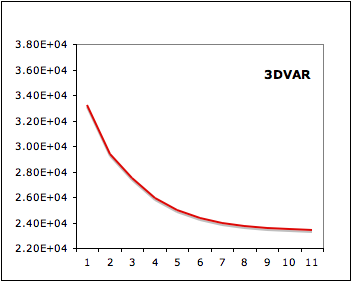
\includegraphics[scale=0.40, trim=10 5 10 20, clip]{3dvar_j} & 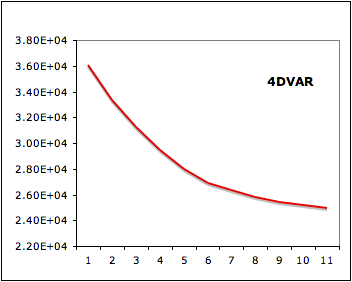
\includegraphics[scale=0.40, trim=10 10 10 20, clip]{4dvar_j}
\end{tabular}
}

\frame{
\frametitle{Sample increments comparison -- U, T}
\begin{tabular}{l r}
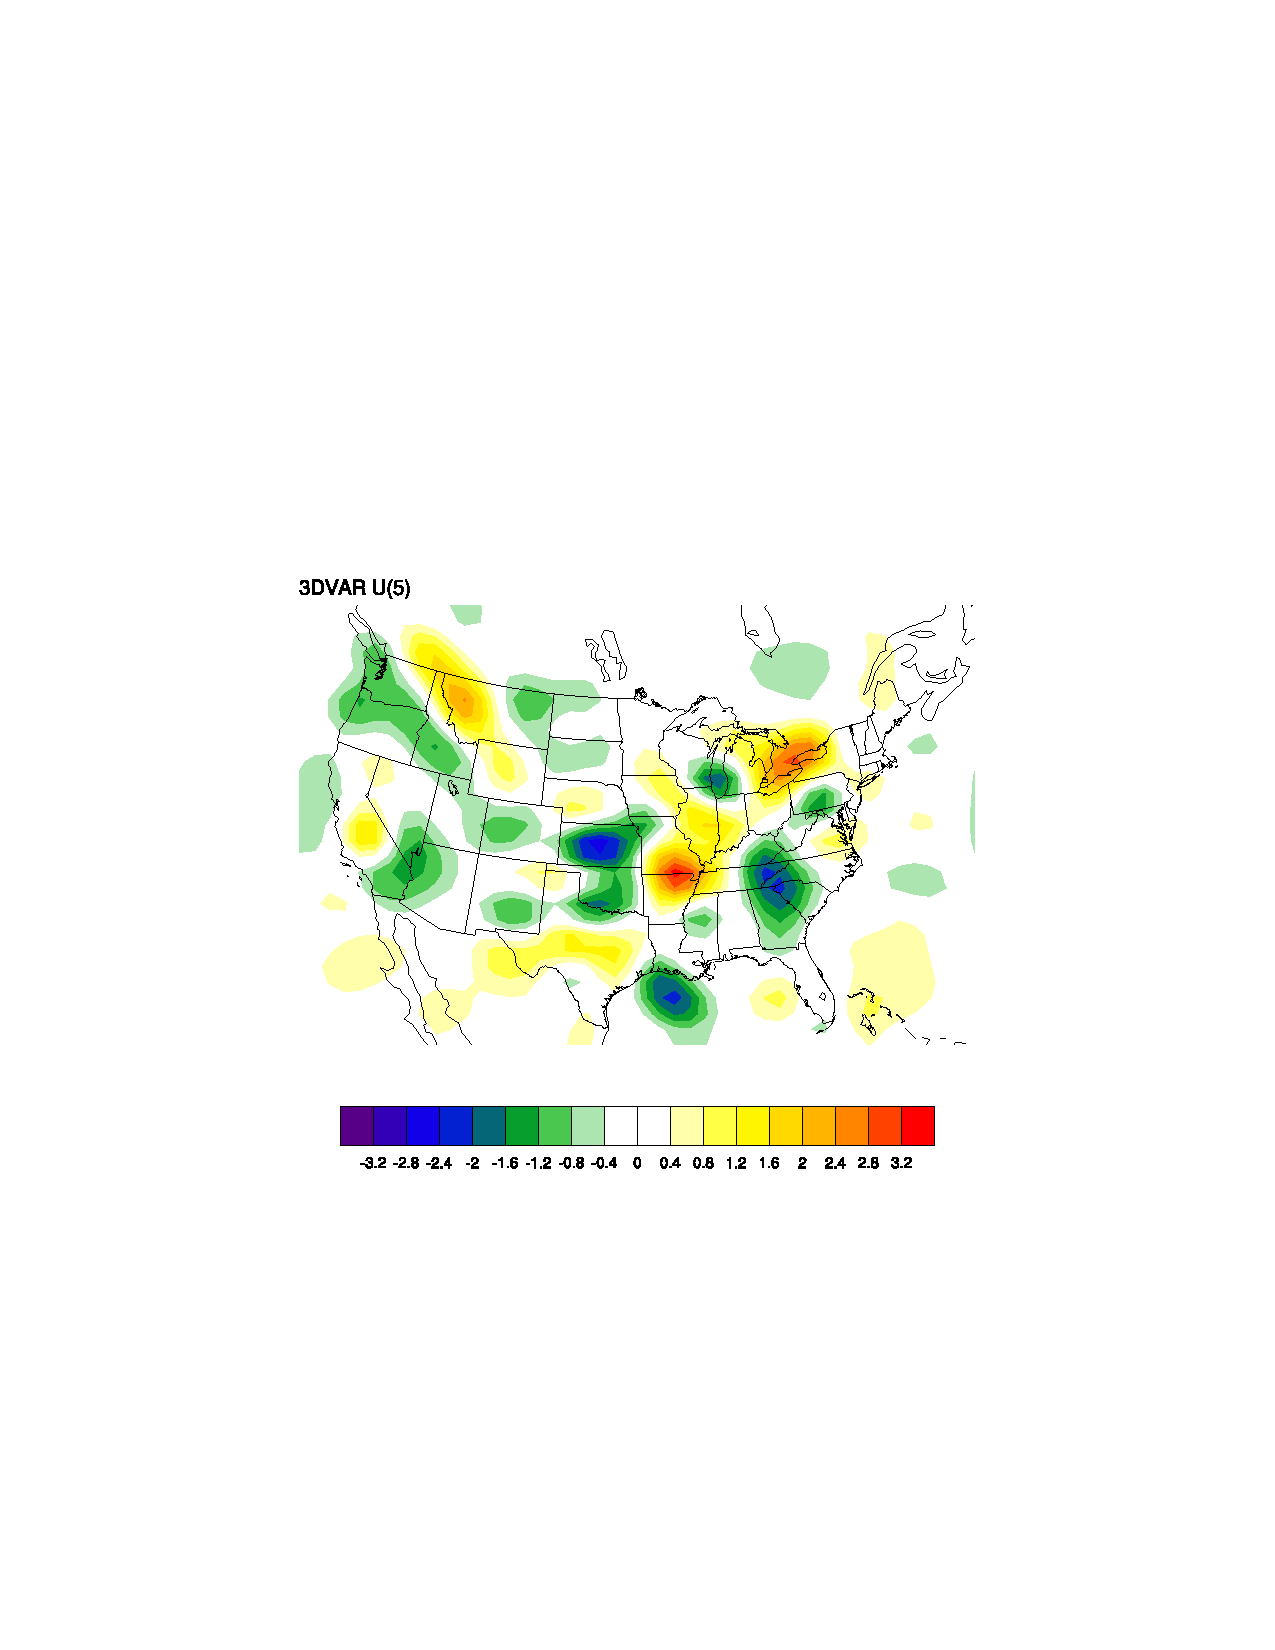
\includegraphics[scale=0.30, trim=50 230 100 250, clip]{3dvar_u_5_inc} & 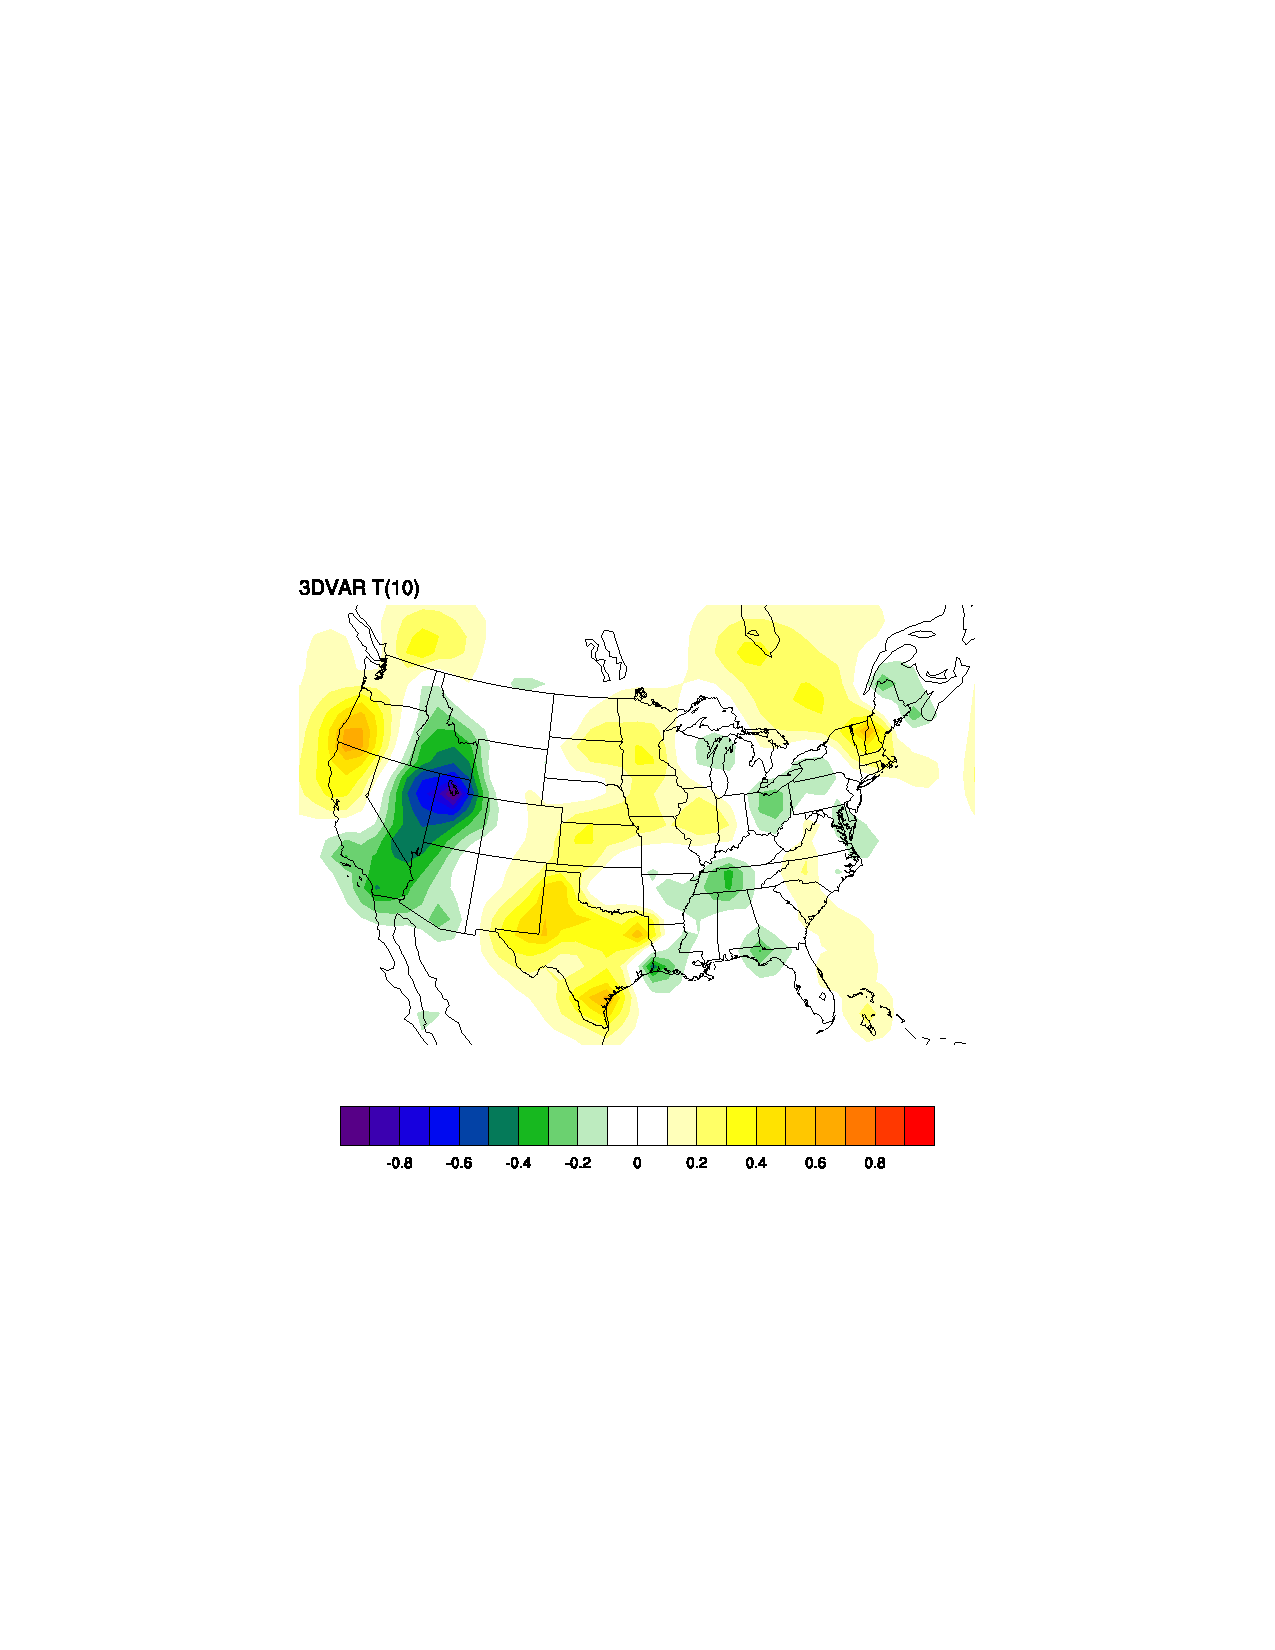
\includegraphics[scale=0.30, trim=100 230 100 250, clip]{3dvar_t_10_inc} \\
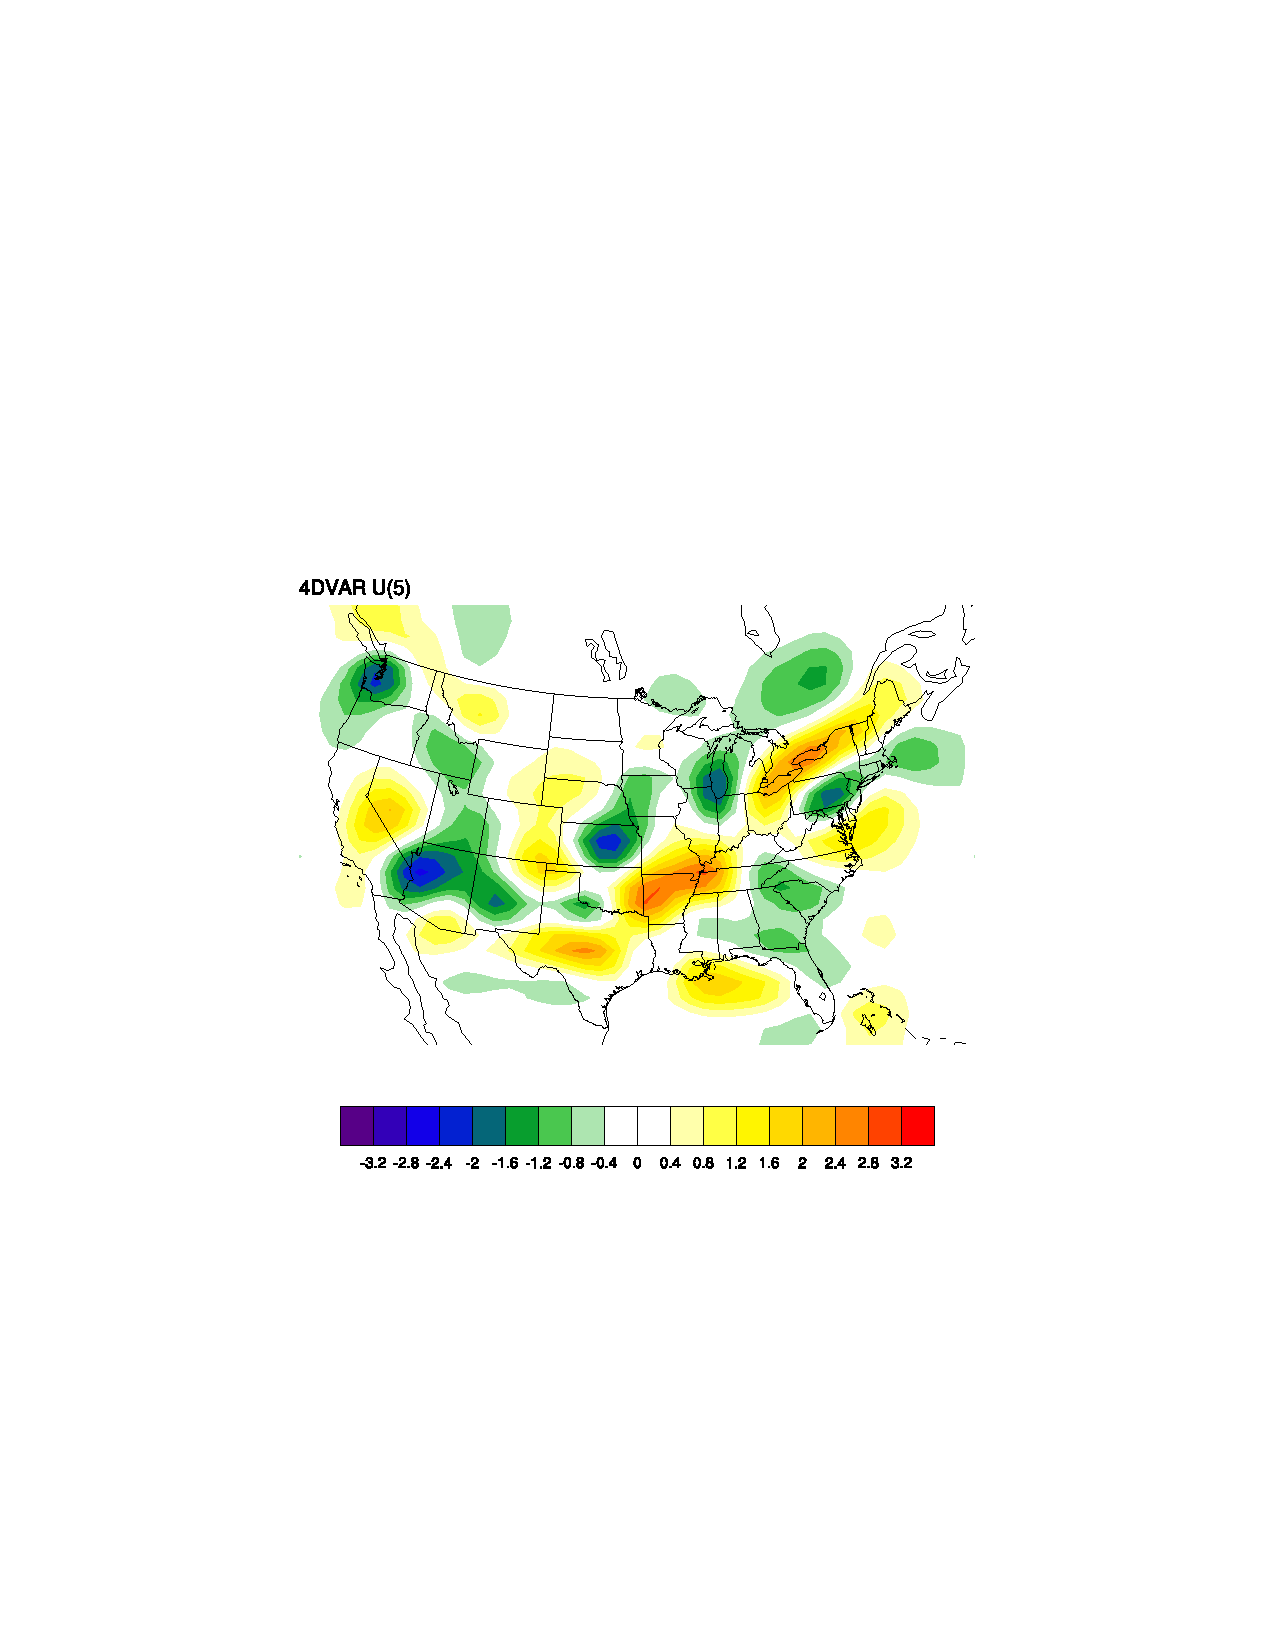
\includegraphics[scale=0.30, trim=50 160 100 250, clip]{4dvar_u_5_inc} & 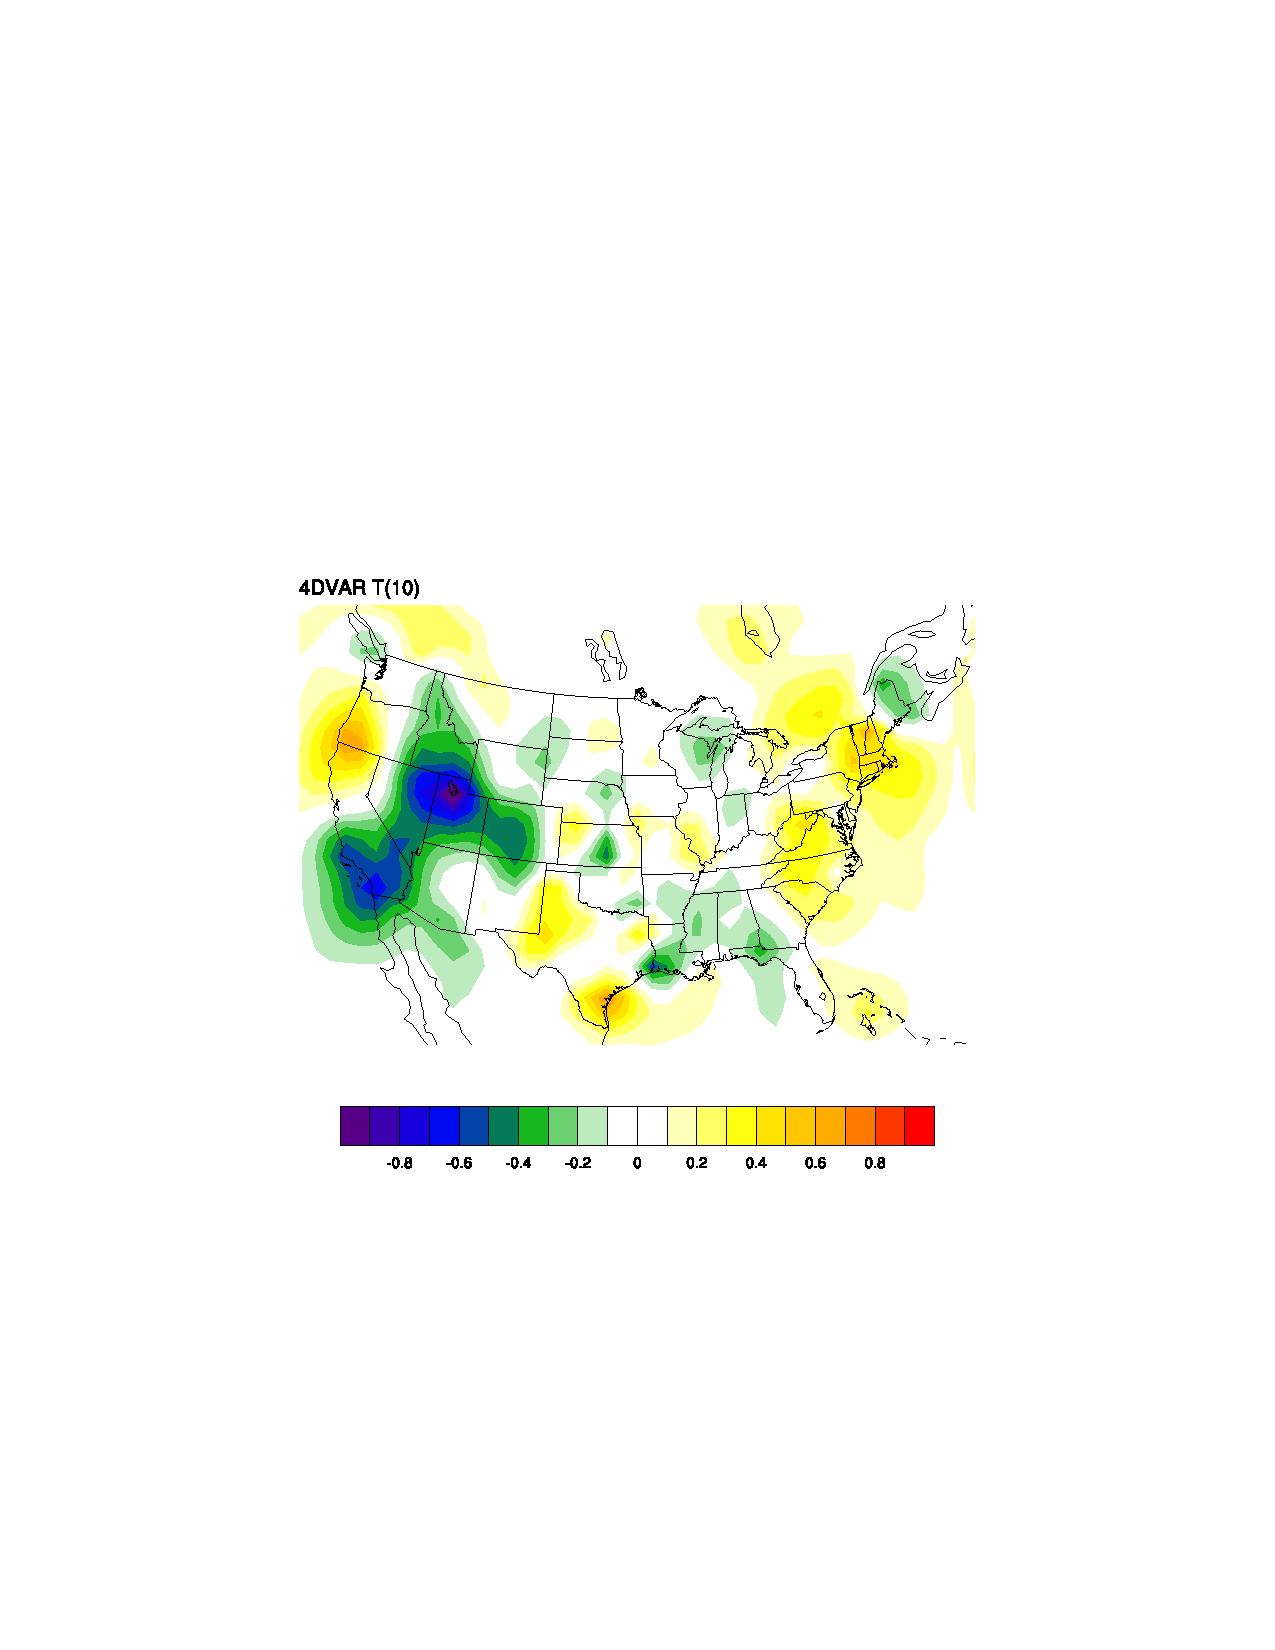
\includegraphics[scale=0.30, trim=100 160 100 250, clip]{4dvar_t_10_inc}
\end{tabular}
}

\frame{
\frametitle{Sample increments comparison -- MU, QVAPOR}
\begin{tabular}{l r}
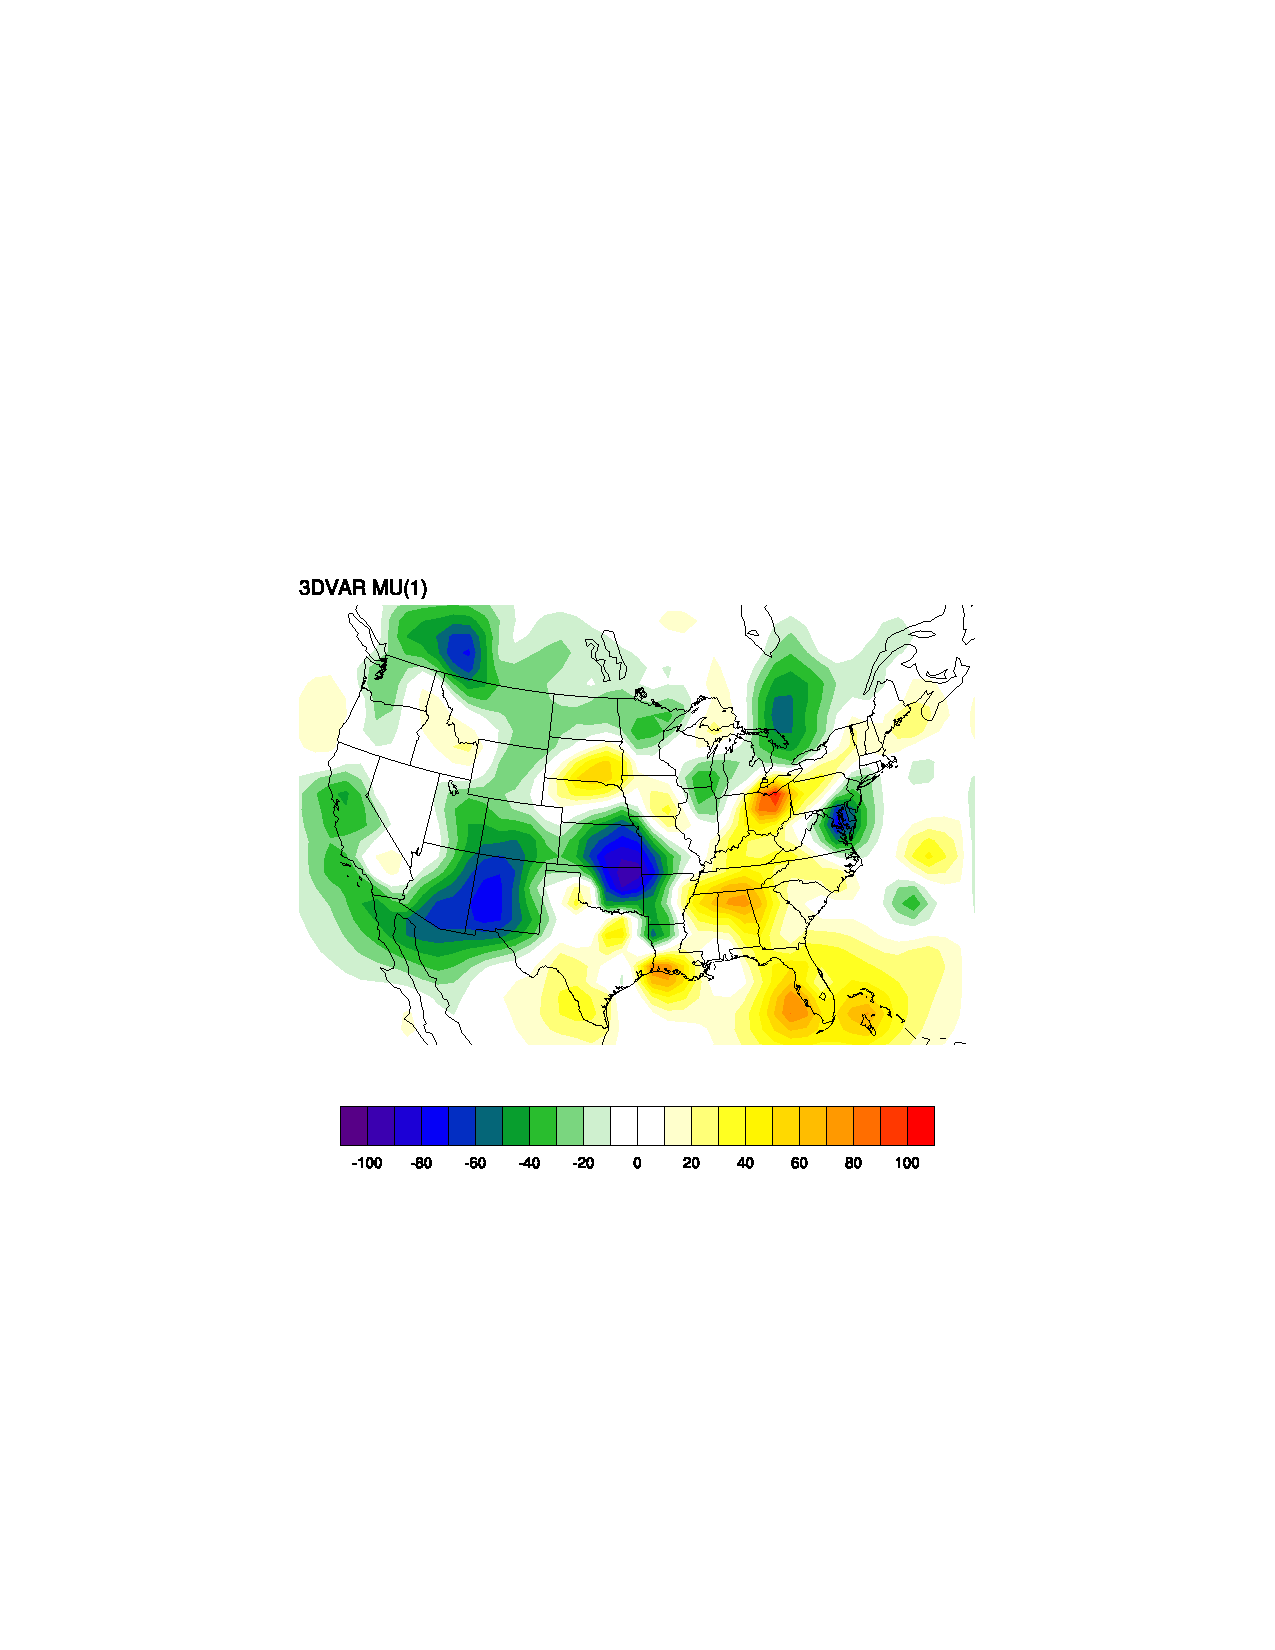
\includegraphics[scale=0.30, trim=50 230 100 250, clip]{3dvar_mu_inc} & 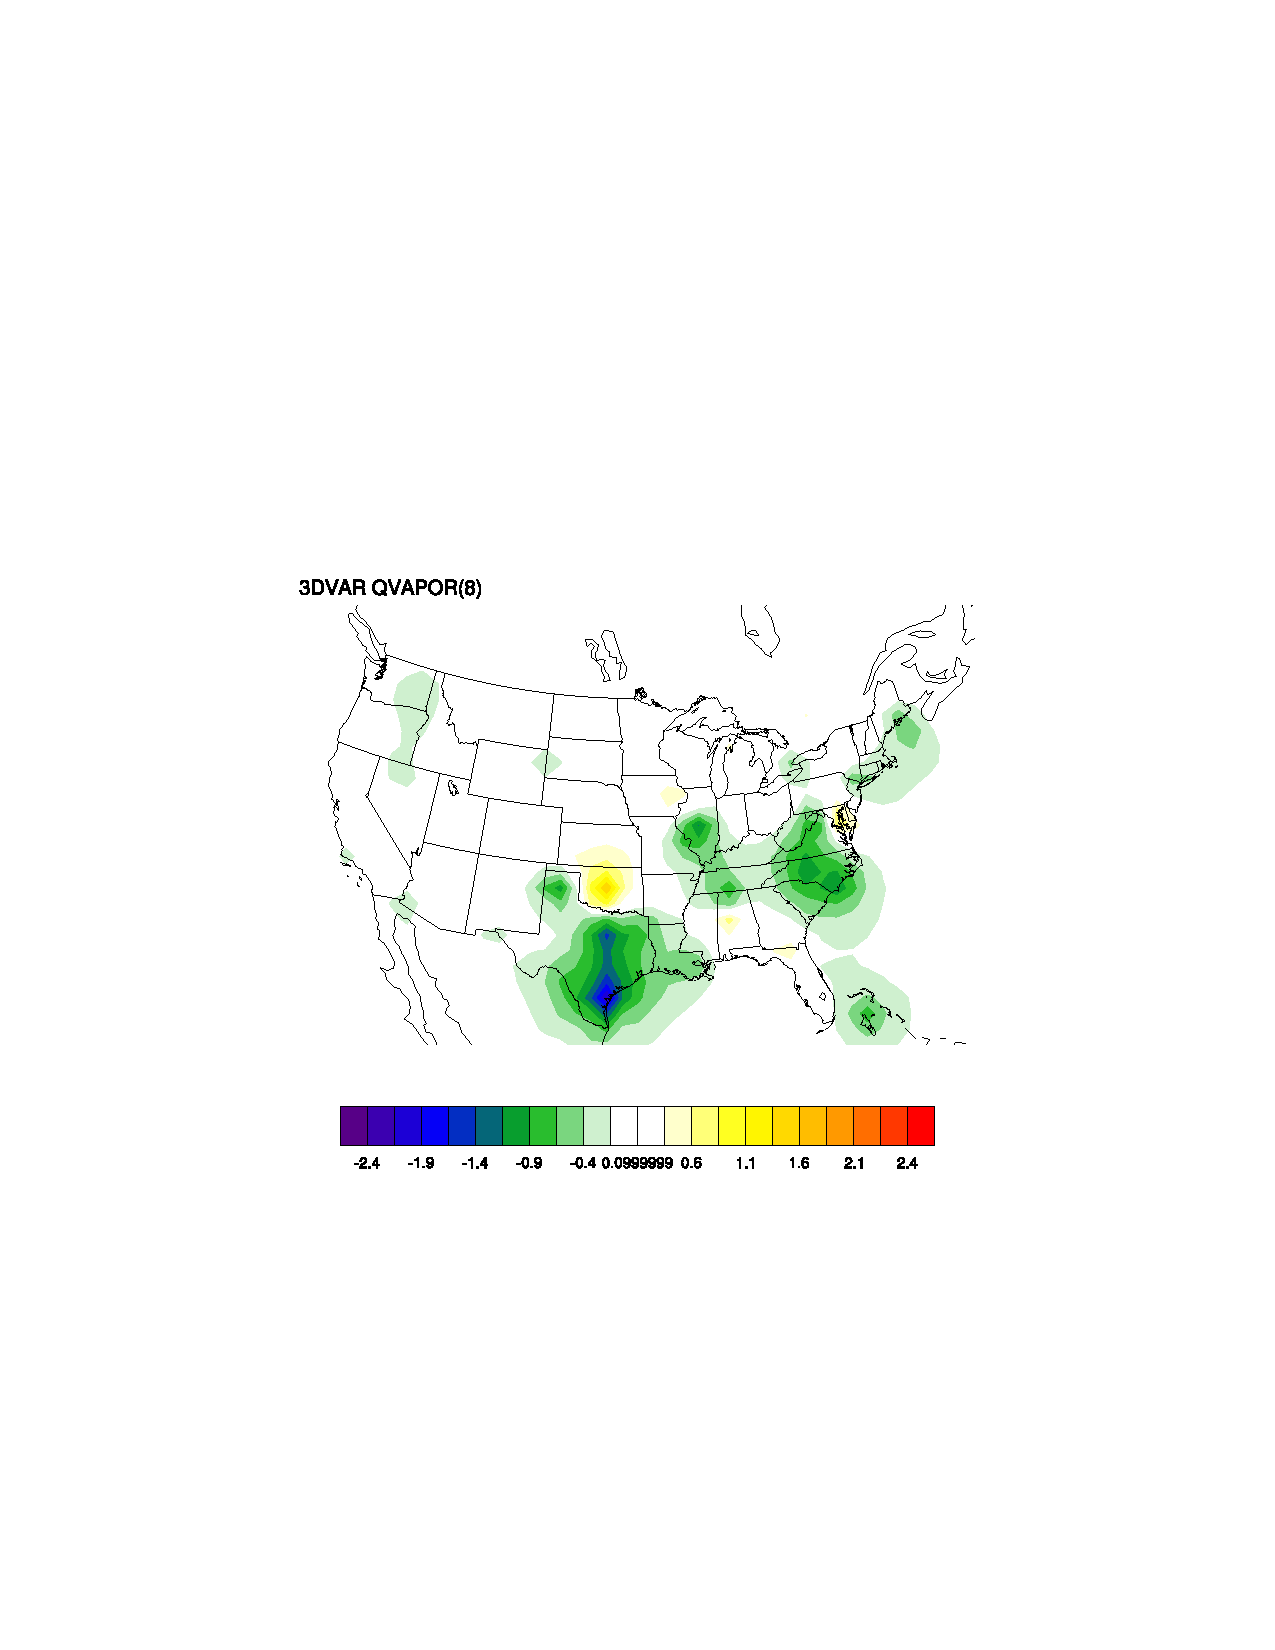
\includegraphics[scale=0.30, trim=100 230 100 250, clip]{3dvar_q_8_inc} \\
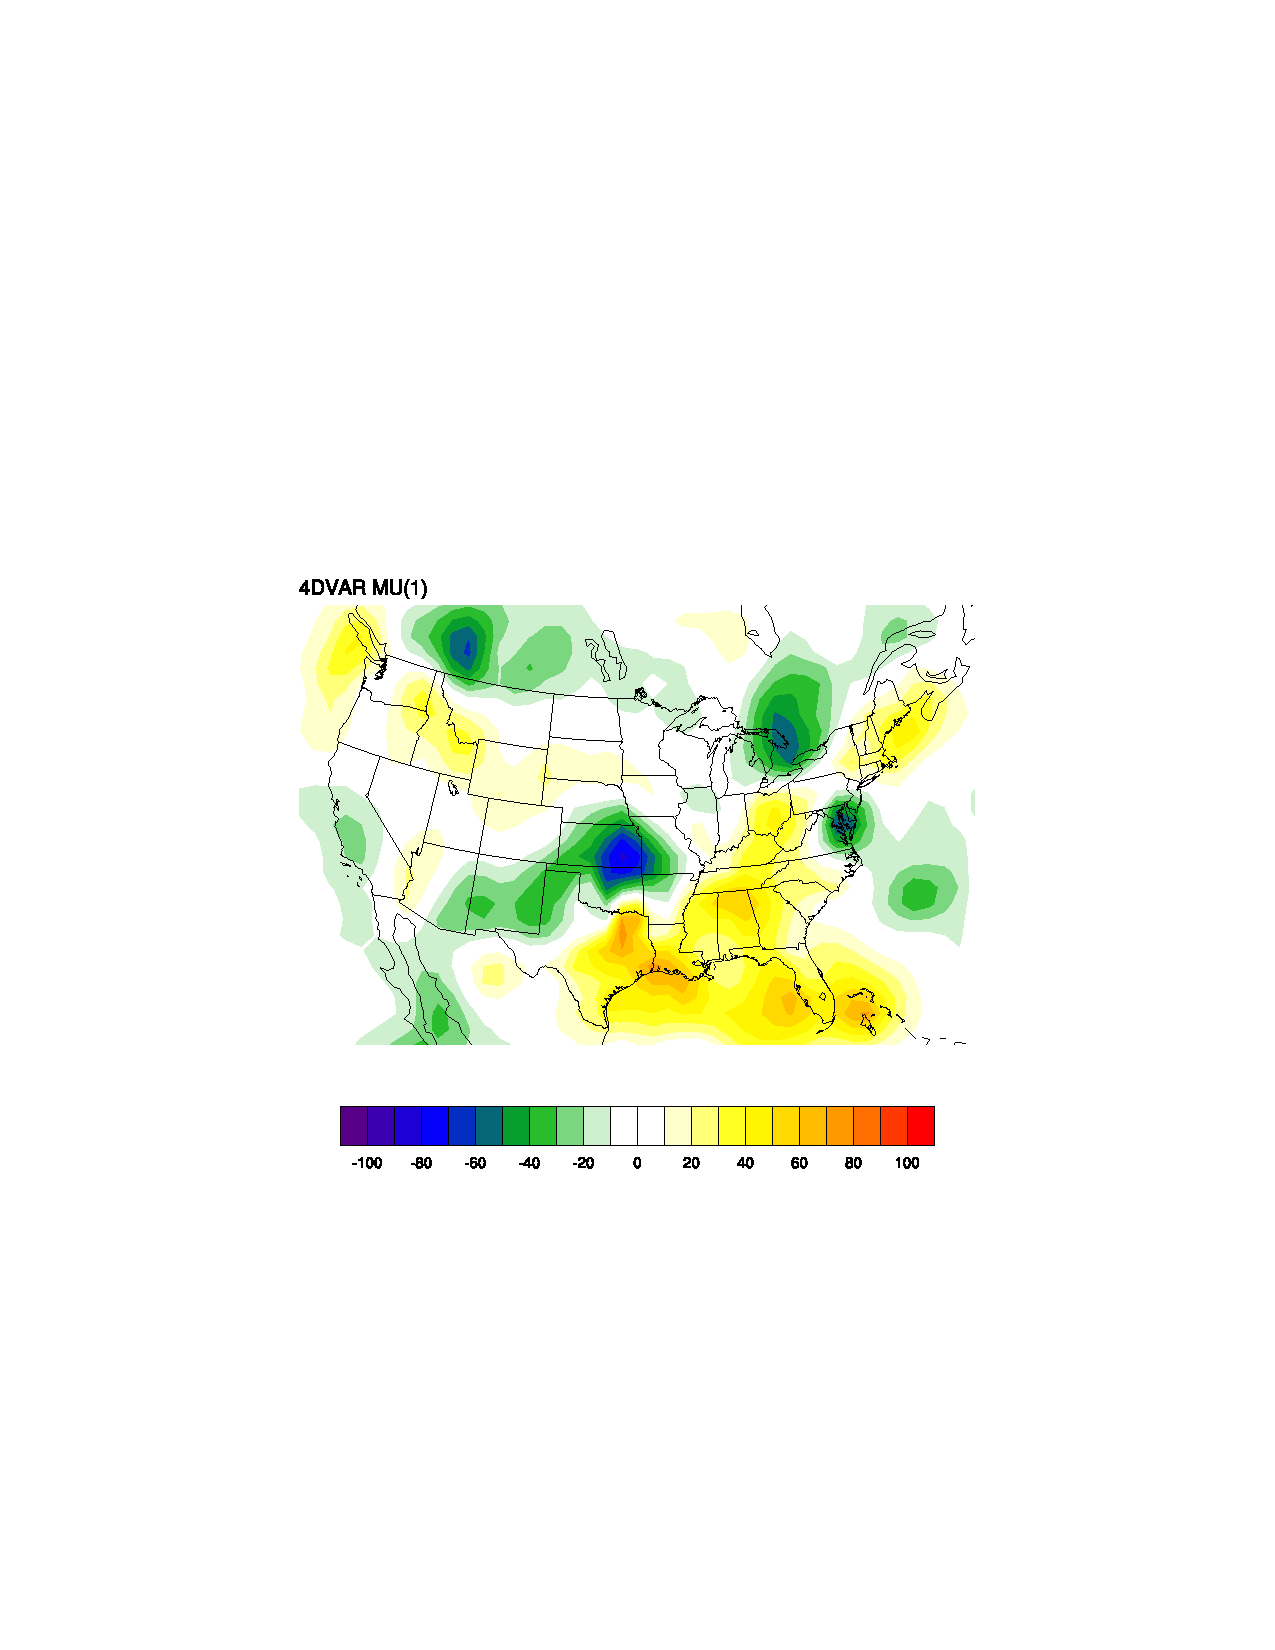
\includegraphics[scale=0.30, trim=50 160 100 250, clip]{4dvar_mu_inc} & 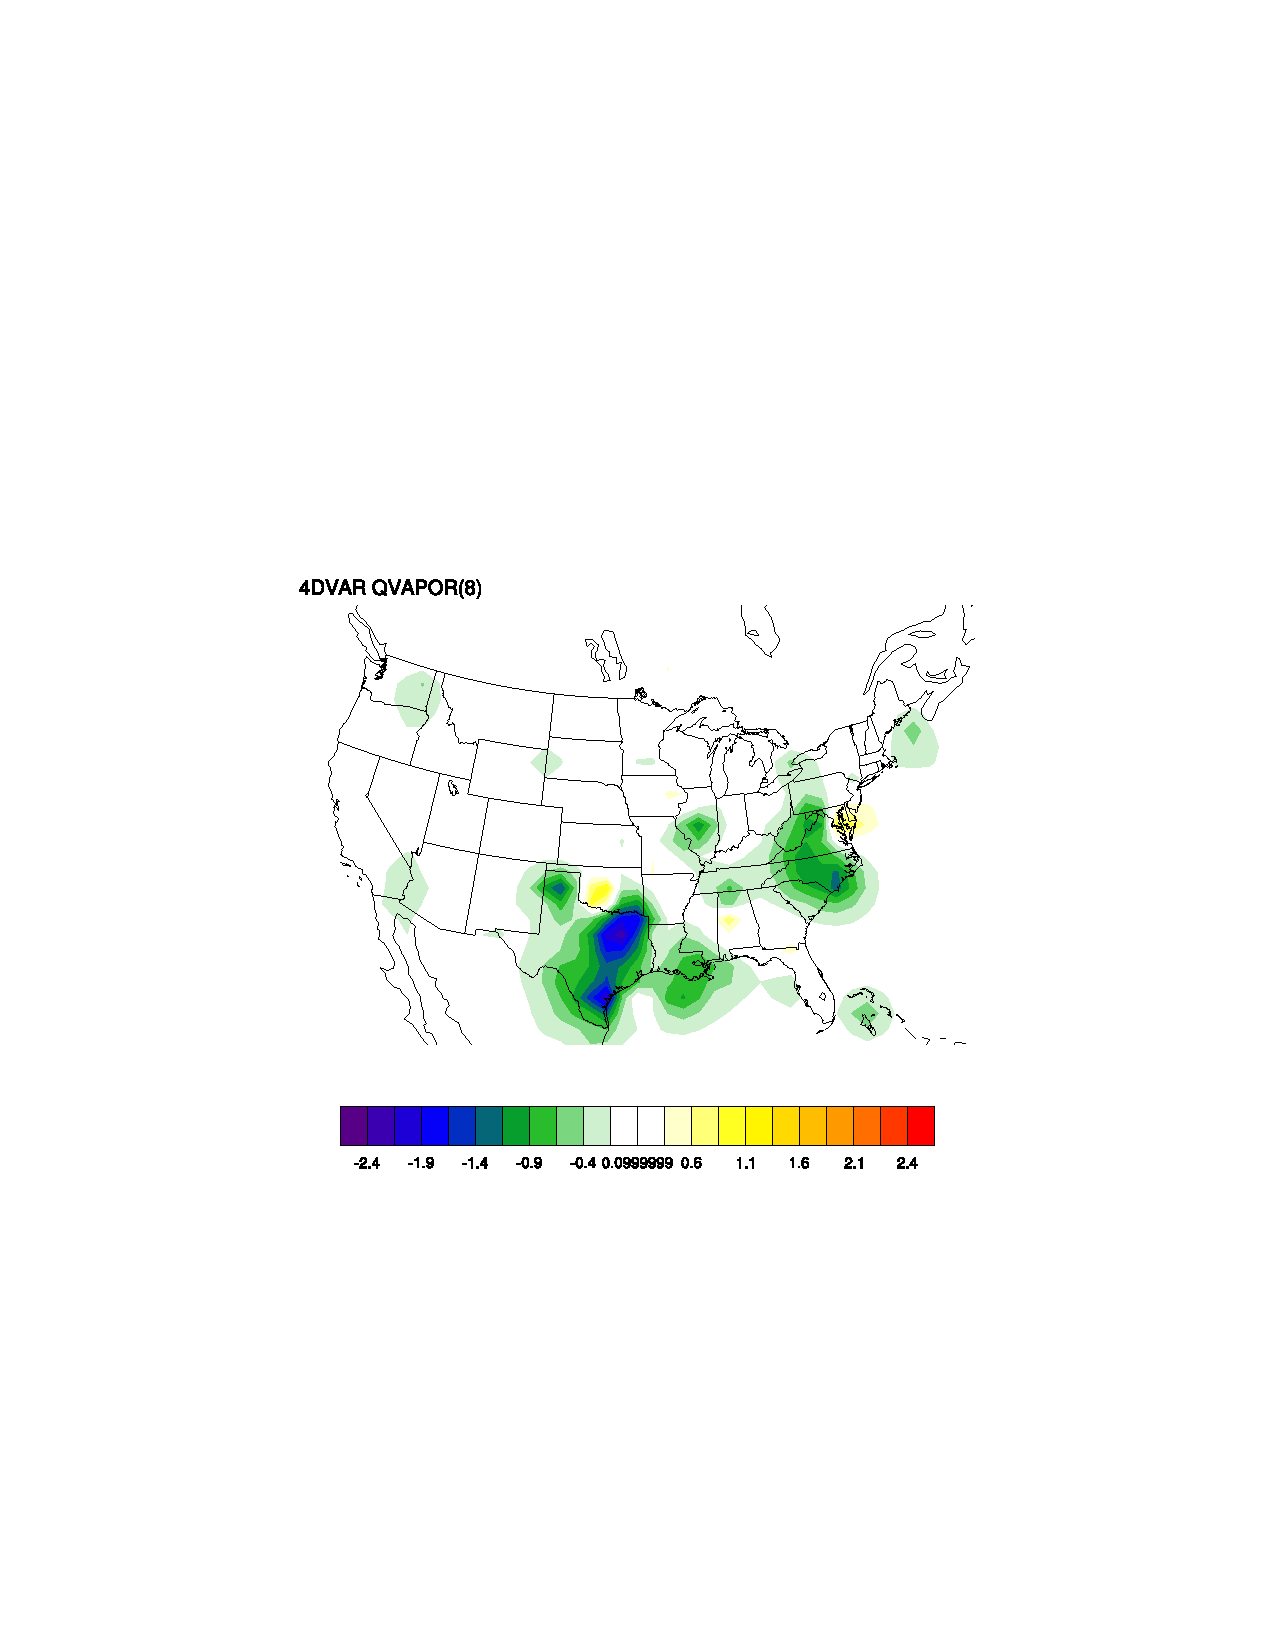
\includegraphics[scale=0.30, trim=100 160 100 250, clip]{4dvar_q_8_inc}
\end{tabular}
}


%%%%%%%%%%%%%%%%%%%%%%%%%%%%%%%%%
\section{Summary}

\frame{
\frametitle{Summary}
\begin{itemize}
	\item The single executable WRF 4DVar system was developed.
	\item Parallelization of WRF tangent linear code has been done.
	\item The new WRF 4DVar system has the capability to assimilate conventional observational data (little\_r or prepbufr format),radiance in bufr format and radar data.
	\item The new WRF 4DVar system is able to consider lateral boundary condition as control variable and digital filter can be used as a weak constraint to suppress the high frequency noise.
\end{itemize}
}

\frame{
\frametitle{Under development}
\begin{itemize}
	\item Add simplified physics packages into WRFPLUS: surface drag, large scale condensation, a simplified moist cumulus scheme, as well as a radiation scheme.
	\item Parallelization of WRF adjoint codes.
\end{itemize}
}

\begin{frame}[fragile]
\frametitle{Quick Start}
Install WRFPLUS and GSI
   \begin{itemize}
        	\item WRFPLUS : WRF adjoint and tangent linear codes
		\begin{verbatim}
	         > configure [-d] wrfplus
	         > compile em_real
	         \end{verbatim}
	\item Set the the $WRF\_DIR$ environmental variable
		\begin{verbatim} 
		> setenv WRF_DIR full_path_of_wrfplus  
		\end{verbatim}
	\item GSI
		\begin{verbatim}
		> configure
		> compile
		\end{verbatim}
    \end{itemize}
\end{frame}

%%%%%%%%%%%%%%%%%%%%%%%%%%%%%%%%%%%
\fst{}{
\begin{center}
~\\
~\\
~\\
~\\
~\\
{\huge{\color{red}Thank You}}\\
~\\
~\\
~\\
~\\
~\\
{\tiny{\color{blue}The NESL Mission is: \\
To advance understanding of weather, climate, atmospheric composition and processes;\\
To provide facility support to the wider community; and, \\
To apply the results to benefit society.\\}}
~\\
{\small{NCAR is sponsored by the National Science Foundation}}
\end{center}
}

\end{document}
